\section{Results}
\label{sec:results}

\subsection{RQ1: continuation likelihoods are robust, but direct judgments are mixed}
Every model shows a positive ignorance gap (Table~\ref{tab:rq1-behavior}). Critical items increase continuation surprisal by 1.856--3.165 summed nats relative to matched controls. Pairwise accuracy ranges from 0.873 to 0.933, and row-level ROC-AUC ranges from 0.722 to 0.821. Thus, after a context supports an explanation, the continuation \emph{and I don't know why} becomes reliably less expected even though the model is never directly asked whether the factor is causal.

The explicit-happenstance diagnostic is positive in all seven models as well. The critical-minus-control advantage for placing the same factor after \emph{because} rather than \emph{and it so happened that} ranges from 0.280 to 0.454 mean token log-probability units. Pairwise accuracy ranges from 0.760 to 0.940 and ROC-AUC from 0.750 to 0.907. Every pair-bootstrap interval excludes zero; all one-sided sign-flip tests attain the Monte Carlo floor ($p=10^{-4}$). This result specifically concerns the explicit happenstance continuation, not a comparison with bare \emph{and}.

\begin{table*}[t]
\centering
\scriptsize
\resizebox{\textwidth}{!}{%
\begin{tabular}{lcccccc}
\toprule
& \multicolumn{3}{c}{IDK} & \multicolumn{3}{c}{Because vs. And} \\
\cmidrule(lr){2-4}\cmidrule(lr){5-7}
Model & Logprob Diff $\pm$ 95\% CI & Pair acc. & AUC & Logprob Diff $\pm$ 95\% CI & Pair acc. & AUC \\
\midrule
Gemma 2 2B   & 2.473 $\pm$ .358 & .887 & .737 & .454 $\pm$ .063 & .940 & .894 \\
Gemma 2 9B   & 3.165 $\pm$ .386 & .927 & .782 & .411 $\pm$ .054 & .927 & .875 \\
Qwen3 4B     & 2.371 $\pm$ .334 & .873 & .758 & .403 $\pm$ .063 & .867 & .845 \\
Qwen3 8B     & 2.914 $\pm$ .373 & .893 & .821 & .280 $\pm$ .063 & .760 & .750 \\
Llama 3.2 3B & 1.856 $\pm$ .287 & .887 & .722 & .361 $\pm$ .053 & .893 & .860 \\
Llama 3 8B   & 2.997 $\pm$ .301 & .927 & .817 & .399 $\pm$ .047 & .907 & .907 \\
\bottomrule
\end{tabular}}
\caption{Behavioral eliciture diagnostics on 150 matched critical--control pairs. Log-probability differences are mean within-pair critical-minus-control differences; CI values are symmetric half-widths of the 95\% pair-bootstrap intervals. Ignorance uses summed continuation surprisal; explicit happenstance uses the mean factor-token log-probability advantage after \emph{because} versus \emph{and it so happened that}.}
\label{tab:rq1-behavior}
\end{table*}

These two diagnostics converge at the model level, but they test different consequences of an inferred explanation: incompatibility with professed ignorance and relative expectation under causal versus explicitly incidental framing. Their consistent direction establishes an output-level eliciture signature before the prompted and representational analyses below.

Direct prompted judgments provide a more mixed picture (Table~\ref{tab:rq1-direct}). Qwen3 4B and 8B discriminate the conditions strongly under both endpoints: their order-averaged Yes/No ROC-AUC is 0.991 and 0.993, and their Likert ROC-AUC is 0.999 and 1.000, respectively. Gemma 2 9B retains useful rank discrimination (0.860 Yes/No and 0.887 Likert AUC). Gemma 2 2B and both Llama models are substantially weaker, with AUC from 0.601 to 0.669 and paired accuracy from 0.627 to 0.753 across endpoints.

\begin{table*}[t]
\centering
\scriptsize
\resizebox{\textwidth}{!}{%
\begin{tabular}{lrrrr}
\toprule
& \multicolumn{2}{c}{Yes/No order average} & \multicolumn{2}{c}{Likert order average} \\
\cmidrule(lr){2-3}\cmidrule(lr){4-5}
Model & Pair acc. & AUC & Pair acc. & AUC \\
\midrule
Gemma 2 2B   & .680 & .647 & .627 & .601 \\
Gemma 2 9B   & .907 & .860 & .947 & .887 \\
Qwen3 4B     & .987 & .991 & 1.000 & .999 \\
Qwen3 8B     & 1.000 & .993 & 1.000 & 1.000 \\
Llama 3.2 3B & .680 & .624 & .753 & .669 \\
Llama 3 8B   & .633 & .619 & .680 & .622 \\
\bottomrule
\end{tabular}}
\caption{Direct behavioral judgments on the same 300 held-out items. Scores are averaged within item across the Yes-or-No and No-or-Yes orders or across the ascending and reversed Likert anchors before computing the threshold-free pair-accuracy and ROC-AUC measures.}
\label{tab:rq1-direct}
\end{table*}

The contrast between Tables~\ref{tab:rq1-behavior} and~\ref{tab:rq1-direct} is therefore model-dependent rather than uniformly negative. Some models express causal sensitivity directly, but across the model set the more consistent behavioral signature appears indirectly in the likelihood of a downstream sentence: whether an ignorance continuation is expected and whether a factor is favored under causal rather than happenstance framing. This dissociation suggests that implicit causal inference can be present even when a metalinguistic answer interface yields poorly calibrated or order-sensitive decisions.

\subsection{RQ2: causal information is decodable, but temporal transfer is weak}
Across the six models, causal probe ROC-AUC averages 0.992 and causal CAA ROC-AUC averages 0.961. Every causal probe exceeds 0.97 AUC, and paired accuracy is at least 0.987. The result is therefore consistent across model families and is not specific to a learned probe: a single mean-difference direction also discriminates held-out causal items well.

By contrast, temporal-to-causal transfer averages 0.686 AUC for probes and 0.647 for CAA. Figure~\ref{fig:rq2-transfer} shows that transfer varies substantially by model and direction; several transferred CAA scores approach chance. Causal-to-temporal transfer is similarly inconsistent. Temporal precedence is therefore not a reliable linear substitute for graded causal implication, despite the high in-domain causal scores.

\begin{figure*}[t]
\centering
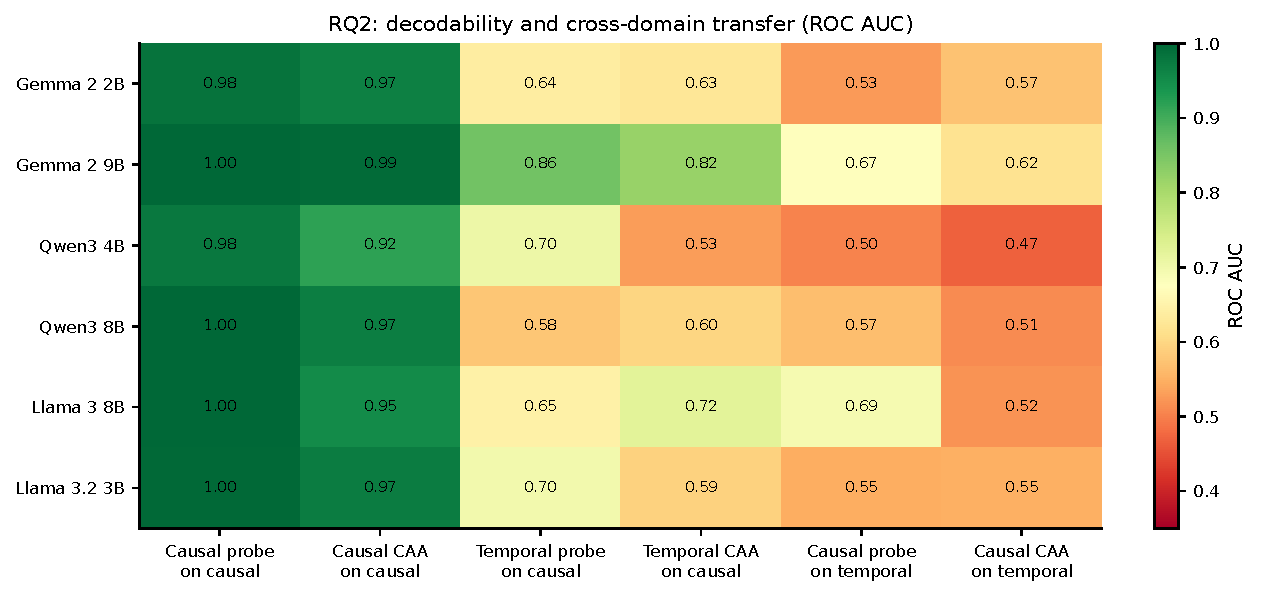
\includegraphics[width=.92\textwidth]{figures/rq1_decodability_transfer.pdf}
\caption{Development-selected probe and CAA ROC-AUC in domain and under causal--temporal transfer. All layers are frozen before test evaluation.}
\label{fig:rq2-transfer}
\end{figure*}

High representational discrimination does not guarantee calibrated behavior. Table~\ref{tab:rq1-direct} shows strong direct rank discrimination for Qwen3 4B and 8B but much weaker discrimination for Gemma 2 2B, Llama 3 8B, and Llama 3.2 3B. Fixed-threshold analyses additionally place the latter three near chance in balanced accuracy. Some of these failures are decision-level collapses: Gemma 2 2B predicts positive on 99.7\% of items under Yes-or-No but on 0\% under No-or-Yes, while its AUC remains 0.608 and 0.654, respectively. Llama 3 8B likewise shifts from a 93.7\% to an 11.7\% positive rate when answer order is reversed. Across models, the mean within-model balanced-accuracy range is 0.071 for Yes/No order and 0.046 for Likert anchor order. The rank-based metrics and fixed-threshold metrics thus diagnose different properties: encoded discrimination versus prompt-dependent decision calibration.

\subsection{RQ3: representations track external ratings more consistently than self-ratings}
Table~\ref{tab:rq3-pearson} reports primary row-level Pearson correlations. Probe correlations with a model's own order-averaged behavior are high for Qwen3 4B and 8B (0.785--0.905), moderate for Gemma 2 9B (0.572--0.593), and weak for Gemma 2 2B and both Llama models (0.139--0.262). CAA follows the same broad pattern but is usually weaker than the probe.

\begin{table*}[t]
\centering
\scriptsize
\resizebox{\textwidth}{!}{%
\begin{tabular}{lcccccc}
\toprule
Model & Probe--Y/N & Probe--Likert & Probe--Gemini & CAA--Y/N & CAA--Likert & CAA--Gemini \\
\midrule
Gemma 2 2B & $.199\pm.091$ & $.149\pm.094$ & $.829\pm.029$ & $.181\pm.100$ & $.104\pm.103$ & $.785\pm.032$ \\
Gemma 2 9B & $.572\pm.067$ & $.593\pm.057$ & $.922\pm.016$ & $.548\pm.076$ & $.567\pm.069$ & $.840\pm.026$ \\
Qwen3 4B & $.785\pm.034$ & $.806\pm.031$ & $.796\pm.036$ & $.656\pm.054$ & $.712\pm.040$ & $.692\pm.044$ \\
Qwen3 8B & $.879\pm.022$ & $.905\pm.015$ & $.889\pm.022$ & $.765\pm.034$ & $.793\pm.034$ & $.774\pm.041$ \\
Llama 3 8B & $.139\pm.081$ & $.204\pm.082$ & $.912\pm.014$ & $.056\pm.091$ & $.244\pm.089$ & $.761\pm.038$ \\
Llama 3.2 3B & $.239\pm.080$ & $.262\pm.077$ & $.871\pm.024$ & $.245\pm.087$ & $.219\pm.093$ & $.798\pm.031$ \\
\bottomrule
\end{tabular}}
\caption{Row-level Pearson correlations, shown as estimate $\pm$ half-width of the pair-clustered 95\% bootstrap interval. Y/N and Likert targets are item-level order averages.}
\label{tab:rq3-pearson}
\end{table*}

In contrast, probe--Gemini correlations range from 0.796 to 0.922, including 0.829 for Gemma 2 2B, 0.912 for Llama 3 8B, and 0.871 for Llama 3.2 3B. These models therefore contain a linearly accessible ordering that agrees with the external graded judgment even when their own final prompted decisions are poorly calibrated. This dissociation argues against interpreting low behavioral balanced accuracy as absence of causal information.

Spearman correlations reproduce the row-level pattern. Pair-difference correlations are considerably smaller: the largest probe Pearson value is 0.38 for Qwen3 4B and 8B, while most Gemini pair-difference correlations are near zero. The strong row-level association is therefore driven mainly by between-item ordering, not by covariation in the magnitude of each critical-minus-control shift. This distinction limits the claim: representations align with graded item plausibility, but do not robustly predict fine-grained paired effect sizes.

\subsection{RQ4: probe-relative failure prediction transfers unevenly}
The prompt-conditioned failure probe is evaluated on 1,200 held-out observations per model. Five of the six models transfer above chance, with balanced accuracies from 0.680 to 0.903 (Table~\ref{tab:rq4-probe}). Gemma 2 2B and Llama 3 8B are strongest at 0.903 and 0.897 balanced accuracy, respectively, and attain macro one-vs-rest AUC above 0.96. Qwen3 8B is the exception: its high overall accuracy (0.917) reflects the dominant correct class, while its balanced accuracy is 0.497 and its post-hoc recall is 0.390. Thus, high causal discrimination in RQ2 does not guarantee that a model's decision failures occupy a stable, linearly transferable state.

\begin{table}[t]
\centering
\small
\resizebox{\columnwidth}{!}{%
\begin{tabular}{lrrrrrrrr}
\toprule
Model & Layer & BAcc & Acc. & AUC & Supp. & Post-hoc & Correct \\
\midrule
Gemma 2 2B   & 17 & .90 & .89 & .96 & .92 & .93 & .86 \\
Gemma 2 9B   & 26 & .78 & .85 & .93 & .88 & .60 & .84 \\
Qwen3 4B     & 28 & .68 & .78 & .84 & .73 & .49 & .81 \\
Qwen3 8B     & 34 & .50 & .92 & .86 & .14 & .39 & .96 \\
Llama 3.2 3B & 13 & .84 & .83 & .93 & .89 & .86 & .78 \\
Llama 3 8B   & 17 & .90 & .88 & .96 & .95 & .90 & .84 \\
\bottomrule
\end{tabular}}
\caption{Frozen three-way probe-relative failure-probe performance on held-out items. Accuracy uses the probe's three-class argmax prediction, without a threshold. AUC is macro one-vs-rest ROC-AUC; the rightmost three columns are class recalls.}
\label{tab:rq4-probe}
\end{table}

\subsection{RQ4: targeted interventions improve some endpoints}
Classifier-gated steering has strongly model- and endpoint-dependent effects (Figure~\ref{fig:rq4-intervention}). The largest Yes/No AUC gains occur for Gemma 2 9B, from 0.830 to 0.985 ($\Delta=0.155$), and Llama 3 8B, from 0.589 to 0.712 ($\Delta=0.123$). Gemma 2 9B Likert improves from 0.866 to 0.919, and Llama 3.2 3B Likert improves from 0.636 to 0.710. The Qwen models show smaller positive changes. Effects need not improve every endpoint: Llama 3 8B Likert falls from 0.567 to 0.473, while Gemma 2 2B changes little.

\begin{figure*}[t]
\centering
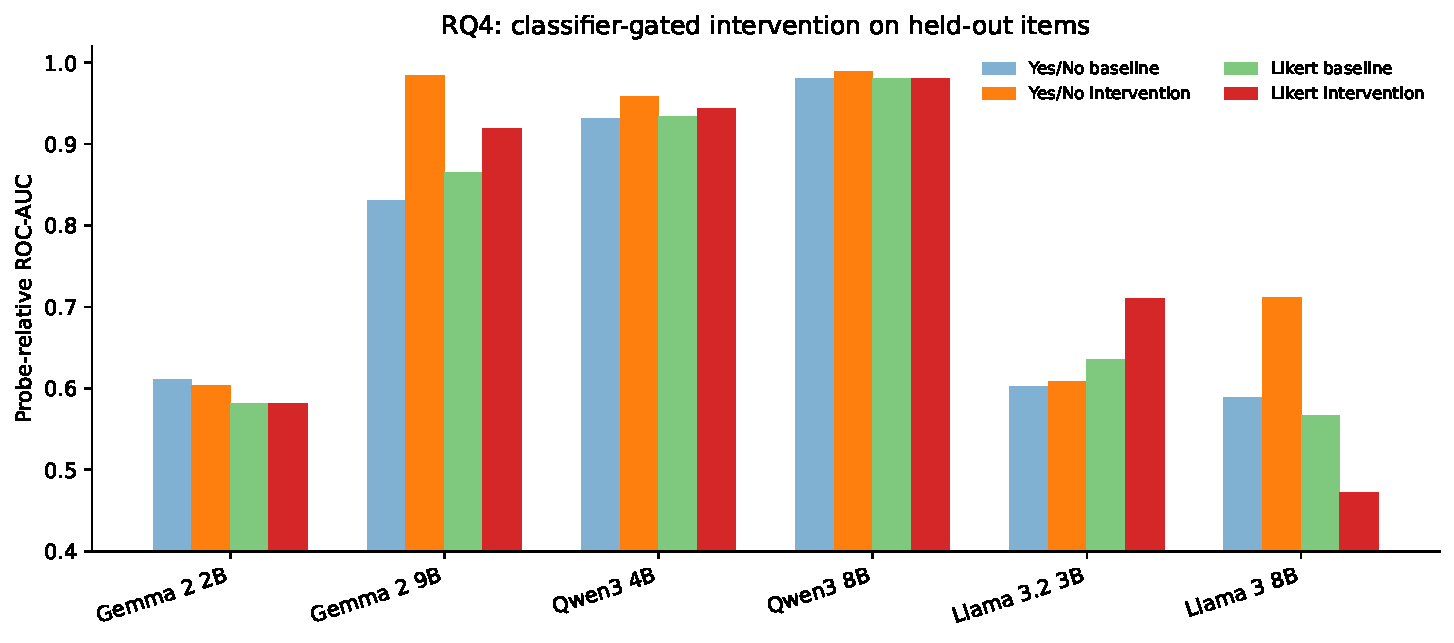
\includegraphics[width=.94\textwidth]{figures/rq4_intervention_auc.pdf}
\caption{Baseline and classifier-gated intervention ROC-AUC against the frozen causal-probe reference on held-out items. Values average the two prompt orders within each endpoint.}
\label{fig:rq4-intervention}
\end{figure*}

Development selection retains $\alpha=0$ when no positive penalized effect is supported, and some endpoint--failure combinations provide no estimable contrast vector. These null selections explain the unchanged aggregate cells. They are informative outcomes under this protocol, not evidence that no nonlinear or more localized intervention could work. More generally, subtracting a failure contrast and observing a predicted output shift provides causal evidence that the selected residual component influences the answer, but does not establish that the vector isolates the full mechanism of causal implication.
